\documentclass[12pt]{article}
\usepackage[left=1cm, right=1cm, top=2cm,bottom=1.5cm]{geometry} 

\usepackage[parfill]{parskip}
\usepackage[utf8]{inputenc}
\usepackage[T2A]{fontenc}
\usepackage[russian]{babel}
\usepackage{enumitem}
\usepackage[normalem]{ulem}
\usepackage{amsfonts, amsmath, amsthm, amssymb, mathtools}
\usepackage{tabularx}
\usepackage{hhline}

\usepackage{accents}
\usepackage{fancyhdr}
\pagestyle{fancy}
\renewcommand{\headrulewidth}{1.5pt}
\renewcommand{\footrulewidth}{1pt}

\usepackage{graphicx}
\usepackage[figurename=Рис.]{caption}
\usepackage{subcaption}
\usepackage{float}

%%Наименование папки откуда забирать изображения
\graphicspath{ {./images/} }

%%Изменение формата для ввода доказательства
\renewcommand{\proofname}{$\square$  \nopunct}
\renewcommand\qedsymbol{$\blacksquare$}

%%Изменение отступа на таблицах
\addto\captionsrussian{%
	\renewcommand{\proofname}{$\square$ \nopunct}%
}
%% Римские цифры
\newcommand{\RN}[1]{%
	\textup{\uppercase\expandafter{\romannumeral#1}}%
}

%% Для удобства записи
\newcommand{\MR}{\mathbb{R}}
\newcommand{\MQ}{\mathbb{Q}}
\newcommand{\MN}{\mathbb{N}}
\newcommand{\MI}{\mathrm{I}}
\newcommand{\MJ}{\mathrm{J}}
\newcommand{\MH}{\mathrm{H}}
\newcommand{\MT}{\mathrm{T}}
\newcommand{\MU}{\mathcal{U}}
\newcommand{\MV}{\mathcal{V}}
\newcommand{\VN}{\varnothing}
\newcommand{\VE}{\varepsilon}

\theoremstyle{definition}
\newtheorem{defn}{Опр:}
\newtheorem{rem}{Rm:}
\newtheorem{prop}{Утв.}
\newtheorem{exrc}{Упр.}
\newtheorem{lemma}{Лемма}
\newtheorem{theorem}{Теорема}
\newtheorem{corollary}{Следствие}

\newenvironment{cusdefn}[1]
{\renewcommand\thedefn{#1}\defn}
{\enddefn}

\DeclareRobustCommand{\divby}{%
	\mathrel{\text{\vbox{\baselineskip.65ex\lineskiplimit0pt\hbox{.}\hbox{.}\hbox{.}}}}%
}
%Короткий минус
\DeclareMathSymbol{\SMN}{\mathbin}{AMSa}{"39}
%Длинная шапка
\newcommand{\overbar}[1]{\mkern 1.5mu\overline{\mkern-1.5mu#1\mkern-1.5mu}\mkern 1.5mu}
%Функция знака
\DeclareMathOperator{\sgn}{sgn}

%Обозначение константы
\DeclareMathOperator{\const}{\text{const}}

%Интеграл в большом формате
\DeclareMathOperator{\dint}{\displaystyle\int}

\newcommand{\smallerrel}[1]{\mathrel{\mathpalette\smallerrelaux{#1}}}
\newcommand{\smallerrelaux}[2]{\raisebox{.1ex}{\scalebox{.75}{$#1#2$}}}

\newcommand{\smallin}{\smallerrel{\in}}
\newcommand{\smallnotin}{\smallerrel{\notin}}

\newcommand*{\medcap}{\mathbin{\scalebox{1.25}{\ensuremath{\cap}}}}%
\newcommand*{\medcup}{\mathbin{\scalebox{1.25}{\ensuremath{\cup}}}}%

%Скалярное произведение
\DeclarePairedDelimiterX{\inner}[2]{\langle}{\rangle}{#1, #2}

%Подпись символов снизу
\newcommand{\ubar}[1]{\underaccent{\bar}{#1}}

\begin{document}
\lhead{Математический анализ - \RN{2}}
\chead{Шапошников С.В.}
\rhead{Лекция - 8}
\section*{Топология точек множества метрического пространства}

\textbf{Вопрос}: Будет ли верно, что $\overline{B(a,r)} = \overline{B}(a,r)$? \textbf{Ответ}: Нет.\\
Например, возьмем $X$ с дискретной метрикой $\Rightarrow B(a,1) = \{a\} = \overline{B(a,1)}$, но $\overline{B}(a,1) = X$.

Такая ситуация возможна только в метрическом пространстве, в нормированном это не так.
\begin{exrc}
	Показать, что в нормированном пространстве $\overline{B(a,r)} = \overline{B}(a,r)$.
\end{exrc}

Надо объяснить, что каждая точка сферы является граничной точкой для открытого шара.
\begin{figure}[H]
	\centering
	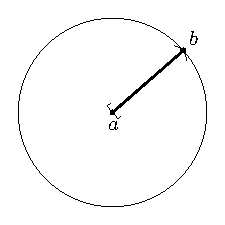
\includegraphics[width=0.25\textwidth]{8_1.eps}
	\caption{Каждая точка сферы - граничная для открытого шара.}
	\label{8_1}
\end{figure}
\uline{Идея}: Берем точки $a + (b-a)t, \, t \in [0,1) \Rightarrow$ будут браться все точки полуинтервала $[a,b)$. Очевидно, что сколь угодно близко к $b$ есть точки открытого шара, но сама точка $b$ не лежит в открытом шаре, а значит это граничная точка. Тогда каждая точка сферы является граничной.
\begin{prop}
	В нормированном пространстве $\overline{B(a,r)} = \overline{B}(a,r)$.
\end{prop}
\begin{proof} Пусть $(X,\|\cdot\|)$ - нормированное пространство, тогда:
	
	$(\Rightarrow)$ Поскольку $\overline{B(a,r)}$ - самое маленькое замкнутое множество, то $\overline{B(a,r)} \subseteq \overline{B}(a,r)$.
	
	$(\Leftarrow)$ Рассмотрим множество $\overline{B}(a,r) = B(a,r) \cup \{\,x \mid \|x - a\|= r \,\},\, B(a,r) \subseteq \overline{B(a,r)}$. Покажем, что множество $A = \{\,x \mid \|x - a\|= r \,\}$ - это множество граничных точек шара $B(a,r)$. 
	
	Пусть $y \in A \Rightarrow$ по условию $ \|y - a\| = r, \, y \in (X \setminus B(a,r))$, тогда:
	\begin{enumerate}[label ={(\arabic*)}]
		\item $\forall B(y,s), \, B(y,s) \cap (X \setminus B(a,r)) \neq \VN$;
		\item Рассмотрим следующее выражение: 
		$$
			x_t = a + (y-a)t,\, t \in [0,1) \Rightarrow \|x_t - a\| = \|a + (y-a)t - a\|= |t|{\cdot}\|y-a\| = |t|{\cdot}r < r
		$$
		так как $t < 1$. Тогда $\forall t \in [0,1), \, x_t \in B(a,r)$. 
		
		Рассмотрим следующиую разницу:
		$$
			\|x_t - y\| = \|a + (y-a)t - y\| = \|(t-1)(y-a)\| = |t-1|{\cdot}\|y-a\| = |1-t|{\cdot}r, \, \forall t \in [0,1)
		$$ 
		таким образом, $\forall s > 0, \exists \, t \in [0,1) \colon |1-t|r < s \Rightarrow x_t \in B(y,s) \Leftrightarrow \forall B(y,s),\, B(y,s) \cap B(a,r) \neq \VN$;
	\end{enumerate}
	Получили, что $\forall y \in A, \, y$ - граничная точка шара $B(a,r) \Rightarrow A \subseteq \overline{B(a,r)} \Rightarrow \overline{B}(a,r) \subseteq \overline{B(a,r)}$.
\end{proof}

Пусть $(X,\rho)$ - метрическое пространство. Возьмем $A \subset X \Rightarrow (A,\rho)$ - метрическое пространство. Как устроены открытые множества в $(A,\rho)$?
\begin{prop}
	$\MU_A$ - открытое множество в $(A,\rho) \Leftrightarrow \exists$ открытое множество $\MU$ в $(X,\rho) \colon \MU_A = \MU \cap A$.
\end{prop}
\begin{figure}[H]
	\centering
	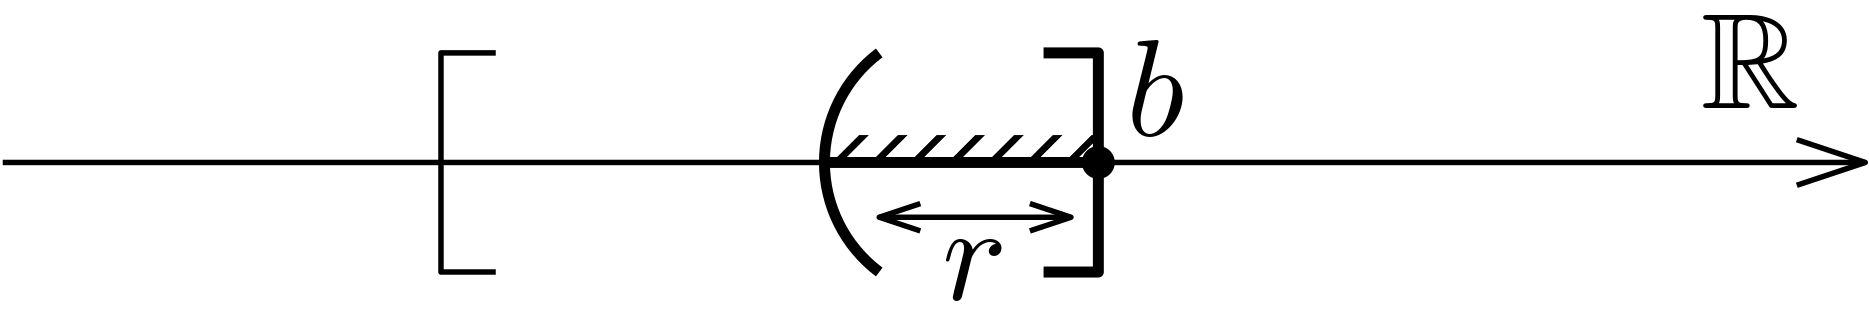
\includegraphics[width=0.4\textwidth]{8_2.png}
	\caption{Открытое множество внутри отрезка (открытый шар $B(b,r)$), но не открытое в $\MR$.}
	\label{8_2}
\end{figure}
\begin{proof}
	Пусть $a \in A$, возьмем шар $B^A(a,r) = \{\, x\in A \mid \rho(a,x) < r \,\} \Rightarrow B^A(a,r) = B(a,r) \cap A$. 
	
	$(\Rightarrow)$ Пусть $\MU_A$ - открытое множество в $A$. Тогда 
	$$
		\MU_A = \textstyle\bigcup\limits_{\alpha} B_\alpha^A = \textstyle\bigcup\limits_{\alpha} (B_\alpha \cap A) = \bigg(\textstyle\bigcup\limits_{\alpha} B_\alpha\bigg) \cap A = \MU \cap A \text{, где } \MU = \textstyle\bigcup\limits_{\alpha} B_\alpha
	$$
	поскольку объединение открытых множеств - открыто. Данное множество $\MU$ предъявляется неоднозначно, но такое множество есть.
	
	$(\Leftarrow)$ Пусть $\exists$ открытое множество $\MU \colon \MU_A = \MU \cap A$, заметим, что всякое открытое множество есть объединение открытых шаров $\Rightarrow$ тогда верны выкладки выше в обратную сторону:
	$$
 		 \MU \cap A =  \bigg(\textstyle\bigcup\limits_{\alpha} B_\alpha\bigg) \cap A = \textstyle\bigcup\limits_{\alpha} (B_\alpha \cap A)  = \textstyle\bigcup\limits_{\alpha} B_\alpha^A = \MU_A 
	$$
	Получили, что $\MU_A$ - открытое множество, как объединение открытых множеств.
\end{proof}
\newpage
\section*{Компакты}

\begin{defn}
	Множество $K \subset X$ в метрическом пространстве $(X,\rho)$, называется \uwave{компактом}, если для всякого набора открытых множеств $\{\MU_\alpha\}$, покрывающих $K$ существует конечный поднабор $\MU_{\alpha_1}, \dotsc, \MU_{\alpha_N}$, покрывающий $K$.
\end{defn}
\begin{defn}
	Множество $\{\MU_\alpha\}$ \uwave{покрывает} $K \Leftrightarrow K \subset \textstyle \bigcup\limits_\alpha \MU_\alpha$.
\end{defn}
\textbf{Пример}: Точка $\{a\}$ - это компакт.

Пусть $K \subset X \Rightarrow (K,\rho)$ - метрическое пространство и открытые множества изменятся. В этом случае $K$ это открытое множество само в себе (знаем, что всё $X$ само в себе это открытое множество). Вдруг $K$ в $X$ это компакт, а само в себе - нет? Или наоборот само в себе компакт, а в $X$ уже нет.

\begin{prop}
	$K\subset X$ - компакт в метрическом пространстве $(X,\rho) \Leftrightarrow K$ - компакт в метрическом пространстве $(K, \rho)$.
\end{prop}
\begin{proof}\hfill\\
	$(\Rightarrow)$ Пусть $K \subset \bigcup\limits_\alpha \MU_\alpha^K$. Знаем, что $\MU_\alpha^K = \MU_\alpha \cap K$, где $\MU_\alpha$ - открытое в $X$. Тогда $K \subset \bigcup\limits_\alpha \MU_\alpha$ в пространстве  в $X$, а в нём, множество $K$ является компактом $\Rightarrow$ можно выбрать конечное подпокрытие 
	$$
		\exists \, \alpha_1, \dotsc, \alpha_N\colon K \subset \textstyle \bigcup\limits_{j = 1}^N \MU_{\alpha_j} \Rightarrow K \subset \textstyle \bigcup\limits_{j = 1}^N (\MU_{\alpha_j} \cap K)
	$$
	по определению пересечения, тогда $K \subset \textstyle \bigcup\limits_{j = 1}^N \MU_{\alpha_j}^K$.
	
	$(\Leftarrow)$ Пусть $K$ - компакт в метрическом пространстве $(K,\rho)$. Тогда можно выбрать конечное подпокрытие $\Rightarrow \exists \, \alpha_1, \dotsc, \alpha_N\colon K \subset \bigcup\limits_{j = 1}^N \MU^K_{\alpha_j} \Rightarrow$ найдутся такие открытые множества $\{\MU_{\alpha_j}\}$ пространства $X$, что по определению открытых множеств в $K$:
	$$
		\MU^K_{\alpha_j} =  \MU_{\alpha_j} \cap K, \, \forall j = \overline{1,N} \Rightarrow K \subset \textstyle \bigcup\limits_{j = 1}^N (\MU_{\alpha_j} \cap K) = \textstyle \bigg(\bigcup\limits_{j = 1}^N \MU_{\alpha_j}\bigg) \cap K \Rightarrow K \subset \bigcup\limits_{j = 1}^N \MU_{\alpha_j}
	$$
	таким образом, получили конечный набор открытых множеств в $X$, покрывающий $K$.
\end{proof}
\begin{lemma}\textbf{(Бореля-Гейне-Лебега в $\MR^n$)}: Брус $[a_1,b_1]\times\dotsc\times[a_n,b_n]$ - является компактом в $\MR^n$ с обычной Евклидовой метрикой.
\end{lemma}
\begin{proof}
	Пусть $n = 2$, докажем с использованием рисунка.
	
	(От противного): Пусть утверждение не верно, тогда найдется покрытие из которого выбрать конечное подпокрытие - нельзя. 
	\begin{enumerate}[label ={(\arabic*)}]
		\item Делим брус на $4$ части, хотя бы у одной из полученных четвертей из данного покрытия нельзя выбрать конечное подпокрытие;
		\item Возьмем полученную четверть, для которой не существует конечного подпокрытия и поделим её опять на $4$ части. Опять найдется четверть у которой нет конечного подпокрытия;
		\item[\vdots] Продолжим аналогичные действия;
	\end{enumerate}
	Получили систему вложенных прямоугольников у которой не существует конечного подпокрытия $\Rightarrow$ по каждой координате мы получили систему вложенных отрезков $\Rightarrow$ по каждой координате есть общая точка (см. первый семестр).
	\begin{figure}[H]
		\centering
		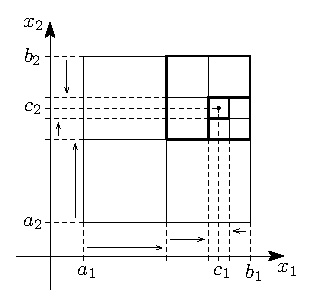
\includegraphics[width=0.3\textwidth]{8_3.eps}
		\caption{Брус $[a_1,b_1]\times [a_2,b_2]$.}
		\label{8_3}
\	\end{figure}
	Тогда 
	$$
		\exists \, c = (c_1,c_2) \in [a_1,b_1]\times [a_2,b_2] \colon c_1 \in [a^n_1, b^n_1], \, c_2 \in [a^n_2, b^n_2], \, \forall n \in \MN
	$$ 
	то есть $c$ принадлежит всем построенным прямоугольникам. Поскольку весь прямоугольник был покрыт открытыми множествами (есть покрытие), то $\exists$ открытое множество $\MU_\alpha\colon c \in \MU_\alpha \wedge \exists \, B(c,r) \subset \MU_\alpha$, поскольку множество открытое и можно внутри него найти шар, покрывающий данную точку.
	\begin{figure}[H]
		\centering
		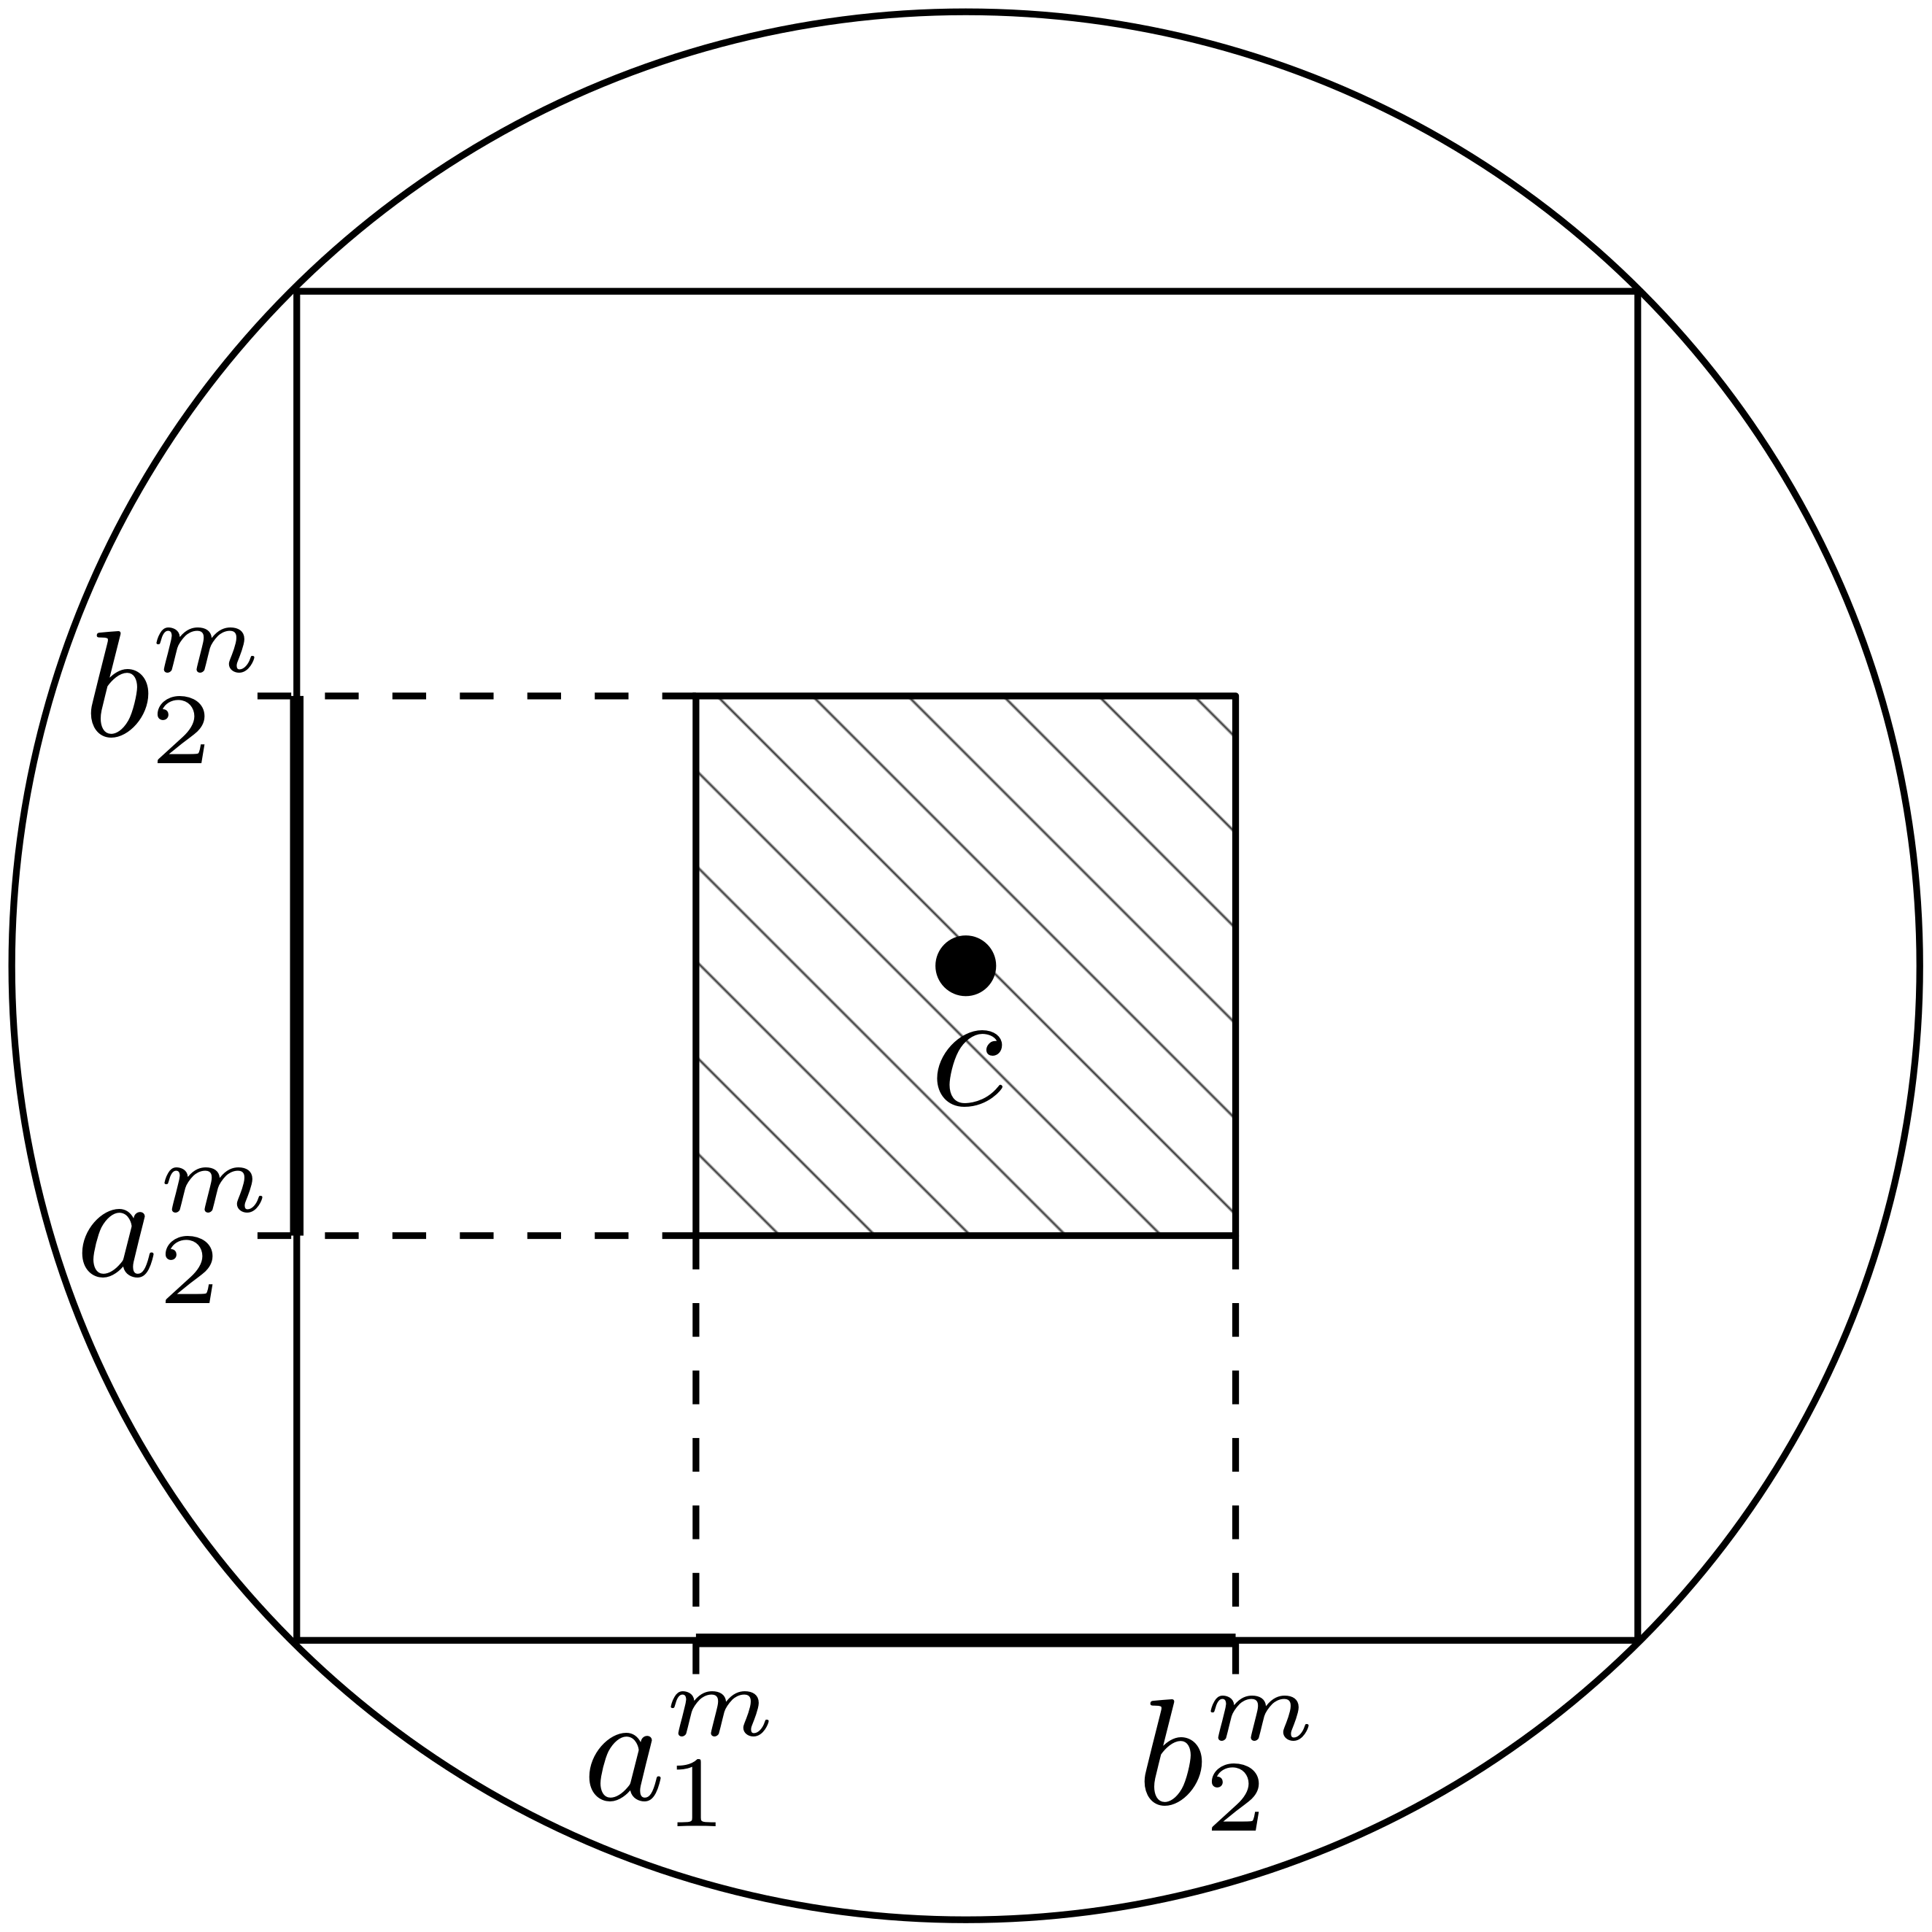
\includegraphics[width=0.25\textwidth]{8_4.png}
		\caption{Прямоугольники внутри открытого шара $B(c,r)$.}
		\label{8_4}
	\end{figure}
	Вписываем в шар прямоугольник, когда проекции вложенных отрезков попадут на стороны этого прямоугольника $\Rightarrow$ построенный прямоугольник целиком попадет внутрь открытого шара $B(c,r) \subset \MU_\alpha \Rightarrow$ противоречие с построением вложенных прямоугольников.
	
	В случае с $n$-мерным кубом, предъявляется шар 
	$$
		B(c,r) = \Big\{\, x \Bigm\vert \sum\limits_{k = 1}^n (x_k - c_k)^2 < r^2 \,\Big\}
	$$ 
	Хотим найти множество вида 
	$$
		C_\delta = [c_1 - \delta, c_1 + \delta]\times \dotsc \times [c_n - \delta, c_n + \delta] \subset B(c,r)
	$$ 
	Какая в этом случае будет $\delta$? Например, $\delta < \tfrac{r}{\sqrt{n}} \Rightarrow$ каждая точка внутри этого множества $C_\delta$ будет $\subset B(c,r)$ и рассуждения будут аналогичны случаю $n=2$.
\end{proof}
\begin{rem}
	Мы вписываем прямоугольник внутрь шара, поскольку таким образом, проще проверять, что другие прямоугольники попали внутрь круга: производим сравнение по сторонам между вписанным прямоугольником и вложенными отрезками.
\end{rem}

\begin{theorem}
	Верны следующие свойства:
	\begin{enumerate}[label ={(\arabic*)}]
		\item Компакт является ограниченным множеством, то есть содержится в шаре; 
		\item Компакт является замкнутым множеством;
		\item Замкнутое подмножество компакта является компактом;
		\item Всякое бесконечное подмножество компакта имеет предельную точку, принадлежащую компакту;
	\end{enumerate}
\end{theorem}
\begin{proof}Доказательства будут аналогичны тем, что рассматривались в первом семестре.
	\begin{enumerate}[label ={(\arabic*)}]
		\item Возьмем точку $a \in X$, построим расширяющиеся шары вокруг неё: $B(a,n), \, \forall n \in \MN$. Тогда всё пространство будет содержаться в объединении этих шаров 
		$$
			X \subset \textstyle \bigcup\limits_n B(a,n) \Rightarrow K \subset X \subset \textstyle \bigcup\limits_n B(a,n)
		$$
		\begin{figure}[H]
			\centering
			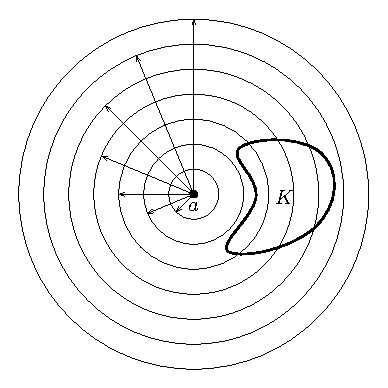
\includegraphics[width=0.35\textwidth]{8_5.eps}
			\caption{Расширяющиеся шары $B(a,n), \, \forall n \in \MN$ и компактное множество $K$ в пространстве $X$.}
			\label{8_5}
		\end{figure}
		Все шары являются открытыми множествами $\Rightarrow$ по определению компакта найдется конечное подпокрытие:
		$$
			\exists \, n_1, \dotsc, n_N \colon K \subset\textstyle \bigcup\limits_{j = 1}^{N} B(a,j)
		$$
		Поскольку шары вложены друг в друга по построению: $B(a,n) \subset B(a,n+1), \, \forall n \in \MN$, то найдем шар в котором содержится весь компакт. Пусть $C = \max\limits_{1 \leq s \leq N}{n_s} \Rightarrow K \subset B(a,C) \Rightarrow K$ - ограниченное множество;		
		\item Если $K$ - замкнутое множество, то его дополнение должно быть открытым. Возьмем точку из дополнения к компакту $a \in X \setminus K$. 
		
		Построим из неё замкнутые шары радиуса $\frac{1}{n}$: $\overline{B}\big(a, \tfrac{1}{n}\big), \, \forall n \in \MN$. Шары являются вложенными 
		$$
			\overline{B}\big(a, \tfrac{1}{n +1}\big) \subset \overline{B}\big(a, \tfrac{1}{n}\big), \, \forall n \in \MN
		$$ 
		дополнения к ним являются открытыми множествами.
		
		Если взять объединение всех этих шаров, то получим объединение открытых множеств, покрывающих все множество $X$ без точки $a$: $\bigcup\limits_n \overline{B}\big(a, \tfrac{1}{n}\big) = X \setminus \{a\}$, поскольку $a\notin K \Rightarrow$ множество $K$ покрывается этим набором $\Rightarrow$ по определению компакта можно выбрать конечное подпокрытие. Тогда 
		$$
			\exists \, \overline{B}\big(a, \tfrac{1}{n_1}\big), \dotsc, \overline{B}\big(a, \tfrac{1}{n_s}\big) \colon K \subset \overline{B}\big(a, \tfrac{1}{n_1}\big)\cup \dotsc \cup \overline{B}\big(a, \tfrac{1}{n_s}\big)
		$$ 
		возьмем самый маленький шарик $\Rightarrow M = \max\limits_{1 \leq s \leq N}{n_s} \Rightarrow K \subset X \setminus\overline{B}\big(a, \tfrac{1}{M}\big)$ - самое большое открытое множество из конечного подпокрытия, содержащее $K \Rightarrow B\big(a, \tfrac{1}{M}\big) \subset \overline{B}\big(a, \tfrac{1}{M}\big) \subset X \setminus K$.
		\begin{figure}[H]
			\centering
			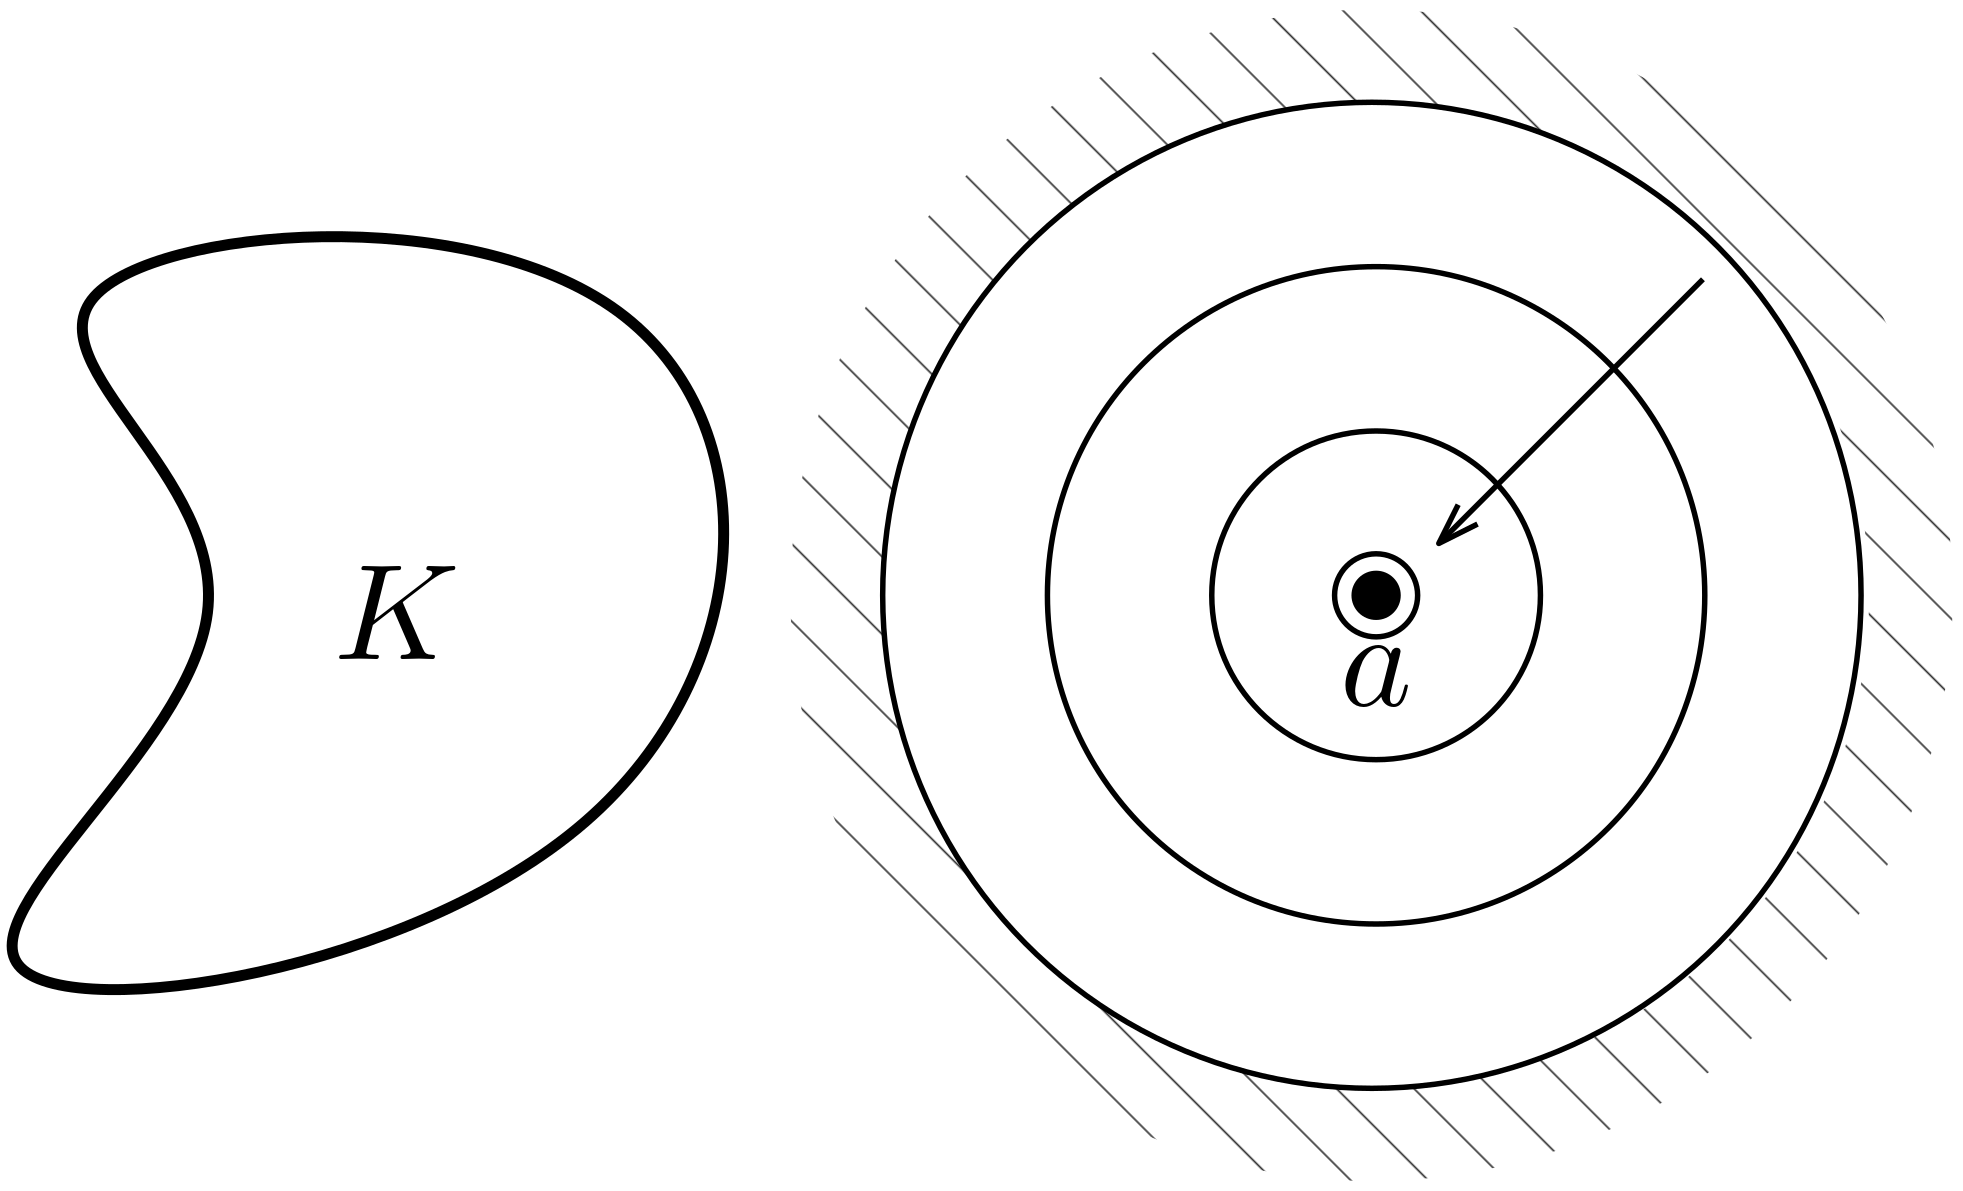
\includegraphics[width=0.35\textwidth]{8_6.png}
			\caption{Дополнение к компакту.}
			\label{8_6}
		\end{figure}
		Таким образом, вместе с каждой точкой дополнение $K$ содержит открытый шар $\Rightarrow$ дополнение множества $K$ - открытое $\Rightarrow K$ - замкнутое множество;
		\item Пусть $F \subset K$ - замкнутое, возьмем покрытие множества $F \Rightarrow F \subset \bigcup\limits_\alpha \MU_\alpha \Rightarrow K \subset \bigcup\limits_\alpha \MU_\alpha \cup (X \setminus F)$. 
		
		Так как $F$ - замкнуто, то $X \setminus F$ - открыто $\Rightarrow$ получили покрытие компакта $\Rightarrow$ возьмем конечное подпокрытие 
		$$
			K \subset \MU_{\alpha_1} \cup \dotsc \cup \MU_{\alpha_N} \cup (X \setminus F)
		$$ 
		но $F\not\subset (X\setminus F) \Rightarrow F \subset \MU_{\alpha_1} \cup \dotsc \cup \MU_{\alpha_N} \Rightarrow$ нашли конечное подпокрытие открытыми множествами для $F$;
		\item (От противного): Пусть $\nexists$ предельных точек бесконечного подмножества компакта, принадлежащих компакту. Тогда $\forall a \in K, \, \exists \, B(a,r)\colon B(a,r)$ содержит конечное множество точек множества $K$. То есть 
		$$
			K \subset \textstyle \bigcup\limits_a B(a,r_a) \Rightarrow K \subset B(a_1,r_{a_1}) \cup \dotsc \cup B(a_N, r_{a_N})
		$$ 
		по определению компакта. Но мы знаем, что в каждом из таких шаров находится конечное множество точек $\Rightarrow$ исходное множество $K$ - конечно $\Rightarrow$ противоречие. 	 	
	\end{enumerate}
	
\end{proof}

\section*{Критерии компактности}

\begin{corollary}(\textbf{Критерий компактности в $\MR^n$})
	$K\subset \MR^n$ - компакт $\Leftrightarrow K$ ограничено и замкнуто.
\end{corollary}
\begin{proof}\hfill\\
	$(\Rightarrow)$ По теореме выше, компакт это ограниченное и замкнутое множество.
	
	$(\Leftarrow)$ Если $K$ - ограничено и замкнуто, то $K$ лежит внутри бруса. По лемме Гейне-Бореля-Лебега, брус это компакт. 
	\begin{figure}[H]
		\centering
		
\includegraphics[width=0.2\textwidth]{8_7.eps}
		\caption{Ограниченное и замкнутое множество лежит внутри бруса.}
		\label{8_7}
	\end{figure}
	Поскольку $K$ это замкнутое подмножество компакта, то по теореме выше $K$ это компакт.
\end{proof}

Когда ограниченное и замкнутое множество не является компактом?

\textbf{Пример}: Пространство $(\MN, \rho)$, где $\rho(x,y) = \begin{cases} 1, & x \neq y \\ 0, & x = y \end{cases}$ - дискретная метрика. Тогда одноточечное множество $\{n\} = B(n,1)$ - это шар радиуса $1$. В этом случае $\MN$ - ограниченное и замкнутое множество:
\begin{itemize}
	\item \textbf{Замкнутость}: $\MN$ - является замкнутым, поскольку все пространство всегда является замкнутым множеством;
	\item \textbf{Ограниченность}: $\MN \subset B(n,2), \, \forall n \in \MN \Rightarrow$ множество ограниченно;
\end{itemize}
Но $\MN$ не является компактом, потому что покрывается своими точками и нельзя выбрать конечное подпокрытие. Часто ли это так или мы просто взяли экзотический пример?

\begin{corollary}
	Из всякой последовательности точек компакта, можно выбрать сходящуюся подпоследовательность к точке компакта.
\end{corollary}
\begin{rem}
	На самом деле верно и обратное $\Rightarrow$ данное свойство равносильно компактности (без доказательства). Данное свойство иногда называют \uwave{секвенциальной компактностью}.
\end{rem}
\begin{rem}
	С компактностью связан термин \uwave{вполне ограниченность}, то есть когда можно компакт покрыть конечным числом шаров с заранее заданным радиусом. Если можно накрыть замкнутое множество в полном пространстве такой ``сеткой'', то это будет компакт.
\end{rem}
\begin{proof}
	Пусть есть последовательность точек $x_n \in K$. Тогда рассмотрим два случая:
	\begin{enumerate}[label ={(\arabic*)}]
		\item Множество значений $x_n$ - бесконечно. Всякое бесконечное подмножество компакта $K$ имеет предельную точку. Пусть для множества значений $x_n$ это $a$. 
		
		Поскольку $a$ это предельная точка, то возьмем шар $B\big(a,\tfrac{1}{k}\big)$ и выберем элементы $x_{n_k} \in B\big(a,\tfrac{1}{k}\big)$ в нём так, чтобы номера $n_1 < n_2 < \dotsc $ были возрастающими. Это возможно, поскольку в каждом таком шаре лежит бесконечно много элементов этого множества, тогда $x_{n_k} \to a$;
		
		\item Множество значений $x_n$ - конечно $\Rightarrow$ какие-то значения повторяются бесконечное число раз: $\exists \, x_{n_k} \equiv a \in K \Rightarrow x_{n_k} \to a$.
		Выбираем подпоследовательность, с элементами, которые повторяют значение и это будет сходящейся подпоследовательностью;
	\end{enumerate}
\end{proof}

\textbf{Пример}: Рассмотрим пространство непрерывных функций $C[0,1]$ и возьмем в нём замкнутое, ограниченное множество 
$$
	\overline{B}(0,1) = \Big\{\,f \colon \max\limits_{[0,1]}|f| \leq 1 \,\Big\}
$$ 
тем не менее данный шар не является компактом.

Предъявим последовательность $f_n$ из которой нельзя выбрать сходящуюся подпоследовательность. Например, такую в которой никакие элементы не сближаются:
\begin{figure}[H]
	\centering
	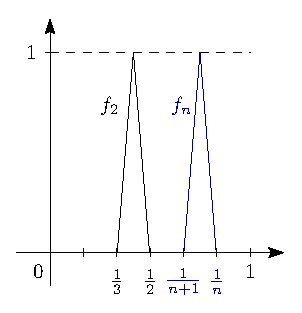
\includegraphics[width=0.3\textwidth]{8_8.eps}
	\caption{Пример ``расставленной'' последовательности $\{f_n\}$.}
	\label{8_8}
\end{figure}
На каждом отрезке будет своя новая функция-зубец $f_n \Rightarrow$ 
$$
	\forall n \neq m, \, \|f_n - f_m\| = \max\limits_{[0,1]}|f_n -f_m| = |1
$$
Тогда никакие две функции не находятся ближе, чем на расстоянии $1$ друг от друга $\Rightarrow$ из $f_n$ нельзя выбрать сходящуюся подпоследовательность.

\newpage
\section*{Компакты в нормированном пространстве}
Рассмотрим нормированные пространства.
\begin{theorem}
	Если в нормированном пространстве, замкнутый шар (положительного радиуса) является компактом, то это пространство конечномерно.
\end{theorem}

\begin{rem}
	Если $\exists$ шар $\overline{B}(a,r), \, r > 0$, который является компактом, то всякий замкнутый шар является компактом.
\end{rem}

Рассмотрим два шара:
$$
	\overline{B(a,r)} = \{\, x \colon \|x - a\| \leq r \,\}, \, \overline{B}(c,R) = \{\, x \colon  \|x - c\| \leq R\}, \, r,R > 0
$$
как получить один шар из другого? 
\begin{enumerate}[label ={(\arabic*)}]
	\item Делаем сдвиг: $x \to x + (c-a)$;
	\item Делаем гомотетию: $x \to \lambda x$, где $ \lambda = \frac{R}{r}$;
\end{enumerate}
Таким образом, всякий шар получается из другого преобразованием параллельного переноса и гомотетии. Сохраняют ли эти операции компактность или нет?

\begin{exrc}
	Показать, что эти операции сохраняют компактность.
\end{exrc}

Далее мы покажем, что непрерывные отображения сохраняют компактность, а эти отображения - непрерывны.
\end{document}